\section{Durchführung}
\label{sec:Durchführung}
\begin{figure}[H]
  \centering
  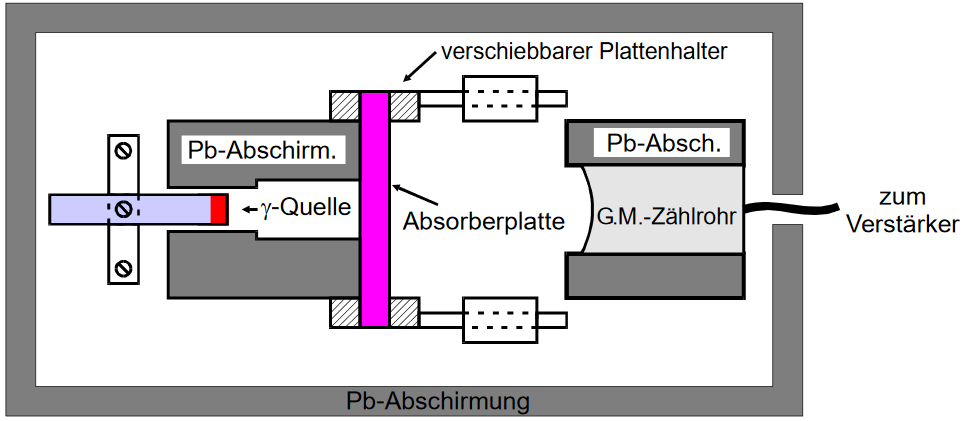
\includegraphics[height=6cm]{Aufbau.PNG}
  \caption{Aufbau der verwendeten Messapparatur. \cite{sample}}
  \label{fig:aufbau}
\end{figure}

Bei dem Versuch wird eine Messapparatur entsprechend Abbildung \ref{fig:aufbau} verwendet.
Zu erkennen ist eine Halterung, in der eine Strahlungsquelle befestigt werden kann.
Das Austreten der Strahlung wird durch eine Bleiabschirmung reguliert. Diese ist nur
in eine Richtung geöffnet, wodurch keine Strahlung zu den Seiten entweichen kann.
In einem gewissen Abstand befindet sich dann ein Plattenhalter, in den man Platten unterschiedlicher
Dicke (wie in diesem Versuch vonnöten) einspannen kann.
Dahinter befindet sich dann ein Geiger-Müller-Zählrohr, mit dem die Intensität der Strahlung gemessen werden kann. Dieser gesamte Aufbau
ist wiederum von einer Bleiabschirmung umgeben, um die Strahlung nach außen hin abzufangen bzw.
um die Apparatur vor äußeren Einflüssen (in Form von Strahlung) zu schützen.

Zu Beginn des
Versuchs der Nulleffekt gemessen. Dabei wird entsprechend noch keine $\gamma$-Quelle eingebaut,
sondern es wird über einen hinreichend langen Zeitraum (900 Sekunden) die Zählrate ohne
jeglichen Einfluss eines extra eingebauten Strahlers gemessen.

Anschließend wird dann eine Quelle eingebaut. Nun wird bei unterschiedlichen Dicken
der Absorberplatte die Zählrate über einen entsprechend langen Zeitraum (je dicker die
Platte, desto länger der Zeitraum) gemessen.

Eine analoge Messung wird anschließend auch für eine $\beta$-Quelle durchgeführt.
